\section{Validation des Fonctions}
Pour effectuer la validation de notre système nous avons téléversé notre projet sur le FPGA, la partie Hardware grâce au SOPC et la partie logicielle à l'aide de l'environnement Eclipse qui nous a permit de lancer/tester et débugger notre projet directement sur la maquette d'évaluation.

\begin{figure}[h]
    \begin{center}
      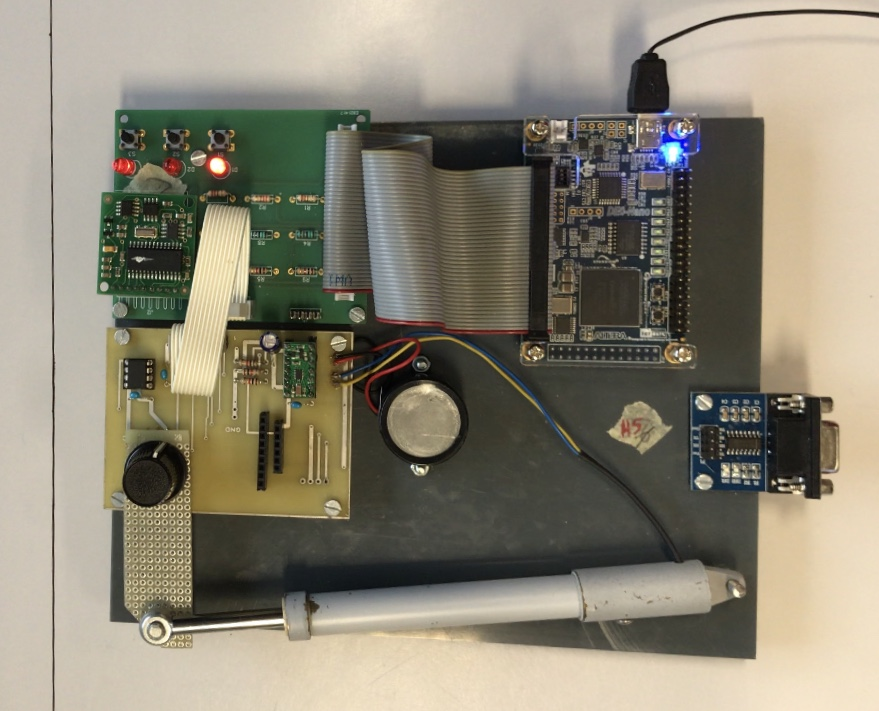
\includegraphics[width=0.7\textwidth]{images/maquette.jpg}
      \caption{Maquette validation projet}
    \end{center}
  \end{figure}

  Nous avons réalisé trois tests pour tester le bon fonctionnement du projet. Pour le premier test nous avons utilisé un GBF qui nous a permit d'injecter directement sur le GPIO, du FPGA attribué, une fréquence qu'on peut modifier pour venir simuler la sortie de l'anémomètre. Après observation la fréquence est bien actualisée toutes les secondes comme demandé dans le cahier des charges. Pour le second test nous venons tester la fonction gestion vérin avec la fonction interface Homme système les boutons nous on permit de tester le bon fonctionnement qui contrôle le signal PWM du vérin. Pour la dernière fonction qui est l'asservissement du système complet nous observons un maintient du cap définit dans le logicielle téléversé sur la maquette de développement et que celle-ci respecte bien le cap fixé avant chaque passage en mode automatique.\newline

  Nous avons aussi testé grâce à l'outil de simulation de Quartus certains composants comme le composant "Div" (Clock\_1Hz), le composant "Detect\_FM" (Détection fronts montants) et la gestion "PWM" important pour la gestion du vérin. Pour cela il faut créer un fichier "Vector Waveform File" et insérer les noeuds que nous souhaitons tester dans l'intervalle de temps, qui doit être adapté pour chaque simulations.
  \newpage
  \subsection{Validation Horloge 1 Hz - Anémomètre}

Une simulation de la fonction "Div" (génération signal 1 Hz) a été réalisée avant implantation, une mesure toute les secondes est nécessaire pour le bon fonctionnement de l'anémomètre c'était donc pour nous une des parties importantes à tester avant de poursuivre le reste du projet.

\begin{figure}[h]
  \begin{center}
    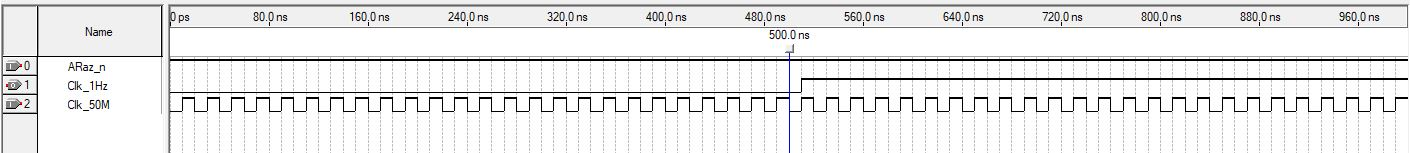
\includegraphics[width=\textwidth]{images/Clk_1Hz.jpg}
    \caption{Simulation du circuit de gestion d'horloge 1 Hz}
  \end{center}
\end{figure}

\subsection{Validation Détecteur Fronts montants - Anémomètre}

Une simulation de la fonction "Detect\_FM" a été réalisée avant implantation, dans cette seconde fonction importante on demande au système de détecter les fronts montants générés par l'anémomètre qui va permettre au système d'informer la vitesse du vent toutes les secondes.

\begin{figure}[h]
  \begin{center}
    \includegraphics[width=\textwidth]{images/Détecteur_Fronts_montants.jpg}
    \caption{Simulation du circuit de détection des fronts montants}
  \end{center}
\end{figure}

\subsection{Validation PWM - Gestion vérin}

Une simulation de la fonction "PWM" a été réalisée avant implantation, dans cette fonction importante de la partie "Gestion vérin" on demande au système de générer un signal PWM qui va être interprété et traité par un composant électronique qui va à son tour piloter le vérin dans un sens ou dans l'autre. Dans cette simulation on observe le bon fonction de celui-ci en faisant varier les valeurs de "Fréquence" et de "Duty".

\begin{figure}[h]
  \begin{center}
    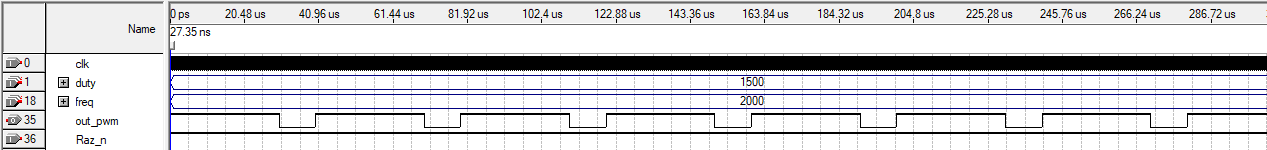
\includegraphics[width=\textwidth]{images/pwm.png}
    \caption{Simulation du circuit de gestion du signal PWM - F = 2000, D = 1500}
  \end{center}
\end{figure}